\documentclass[11pt]{article}
\usepackage[utf8]{inputenc}
\usepackage[T1]{fontenc}
\usepackage{amsmath,amsfonts,amssymb}
\usepackage{amssymb}
\usepackage{multicol}
\usepackage[a4paper,left=2.5cm,right=2.5cm,top=2.5cm,bottom=2.5cm]{geometry}
\usepackage[english]{babel}
\usepackage{libertine}
\usepackage{gensymb}
\usepackage{tabularray}
\usepackage{graphicx}
\usepackage{steinmetz}
\usepackage{wrapfig}
\usepackage{float}
\usepackage{enumitem}
\usepackage[]{titletoc}
\usepackage{nicematrix}
\usepackage{titlesec}
\usepackage{mathtools}
\usepackage{caption}
\usepackage{subcaption}
\usepackage[bottom]{footmisc}
\usepackage{pdfpages}
\usepackage{tabularx}
\titleformat{\chapter}[display]
  {\normalfont\bfseries}{}{0pt}{\Huge}
\usepackage{hyperref}
\newcommand{\hsp}{\hspace{20pt}}
\newcommand{\HRule}{\rule{\linewidth}{0.5mm}}
\newcommand\independent{\protect\mathpalette{\protect\independenT}{\perp}}
\def\independenT#1#2{\mathrel{\rlap{$#1#2$}\mkern2mu{#1#2}}}

\usepackage{apptools}
    \titleformat{\chapter}[hang]{\bfseries\huge}{\IfAppendix{\appendixname~}{\relax}\thechapter\IfAppendix{.}{.}}{\IfAppendix{0.333em}{2pc}}{}

\titlespacing {\chapter}{0pt}{0pt}{40pt}

\usepackage[nottoc]{tocbibind}
\usepackage{graphicx}
\usepackage{float}

\usepackage{keyval}
\usepackage{kvoptions}
\usepackage{fancyvrb}
\usepackage{ifthen}
\usepackage{calc}
\usepackage{pdftexcmds}
\usepackage{etoolbox}
\usepackage{xstring}
\usepackage{xcolor}
\usepackage{lineno}
\usepackage{tikz}
\usepackage{circuitikz}
\usetikzlibrary{patterns,arrows,decorations.pathreplacing,babel}

\usepackage[]{minted}
\newminted{python}{
    linenos=true,
    bgcolor=lightgray,
    tabsize=4,
    gobble=8,
    fontfamily=courier,
    fontsize=\small,
    xleftmargin=5pt,
    xrightmargin=5pt
}
\usepackage[many]{tcolorbox}

\title{LINMA2171 (2024–2025) — Numerical Analysis: Approximation, Interpolation, Integration\\
Homework 1}
\author{Desmidt Simon (\texttt{19012100})}
\begin{document}
\maketitle
\begin{tcolorbox}[breakable,
                  colback=white,
                  colframe=white!75!black,
                  title={A finite set \(\chi \subset \mathbb{R}^d\) is said to be \(\mathcal{P}_n^d\)-unisolvent if the only polynomial \(p \in P_n^d\) which vanishes on \(\chi\), i.e. \(p(x) = 0\) for all \(x \in\chi\), is identically zero. In the univariate case, which sets are \(P^1_n\)-unisolvent ?}
                 ]
    If \(p(x)=0\) for all \(x\in \chi\), it means that each element of \(\chi\) is a zero of the polynomial \(p\). Let \(r\) be the number of real zeros of the polynomial \(p\). Each set of points containing strictly more than \(r\) elements is identically zero, as the polynomial cannot, by definition, have more than \(r\) real zeros. 
\end{tcolorbox}
\begin{tcolorbox}[breakable,
                  colback=white,
                  colframe=white!75!black,
                  title={Show that \(P^d_n\)-unisolvent sets are invariant under affine invertible transformation, that is, if \(\chi\subset \mathbb{R}^d\) is \(P^d_n\)-unisolvent then \(A\chi + b = \{Ax + b | x \in \chi\}\) is also \(P^d_n\)-unisolvent, for any invertible matrix \(A \in \mathbb{R}^{d\times d}\) and \(b \in \mathbb{R}^d\).}
                 ]
    We will work here by contraposition: if there exists a non identically zero polynomial that interpolates \(A\chi+b\), then there exists a non identically zero polynomial that interpolates \(\chi\).\\

    By hypothesis,
    \begin{align}
        \exists p\in \mathcal{P}_n^d \text{ such that } & \exists y'\notin A\chi+b\: : \: p(y')=0\\
        & \forall y \in A\chi +b \: : \: p(y) = 0
    \end{align}
    As \(y=Ax+b\), with \(A\) invertible, \(x=A^{-1}(y-b)\) and we denote \(q(x) = q(A^{-1}(y-b))\in \mathcal{P}_n^d\).\\
    If \(p(Ax+b)=0 \:\forall x\in \chi\), then we can find a polynomial \(q\) such that \(q(x)=0 \:\forall x\in \chi\) by solving for \(y\) \(p(y)=0\), then solving for \(x\) \(x = A^{-1}\)
\end{tcolorbox}
\begin{tcolorbox}[breakable,
                  colback=white,
                  colframe=white!75!black,
                  title={Compute explicitly the dimension of \(P^d_n\). Provide (with proof) a sufficient condition for the existence and the uniqueness of the d-variate polynomial interpolation of degree n at the set of points \(\chi\). Later, if this sufficient condition is satisfied, we will simply say that the interpolation problem is well-posed.}
                 ]
    The number of monomials of degree \(i\) is determined based on the binomial coefficients: for the degree \(i\) of a \(d\)-variate polynomial, the number of terms is \[\frac{(d+i-1)!}{i!(d-1)!}\] Now summing on \(i=0,\dots,n\), for every degree possible for a polynomial of maximum degree \(n\):
    \begin{equation}
        \color{red}\boxed{\color{black}\sum_{i=0}^n \frac{(d+i-1)!}{i!(d-1)!} = \frac{(d+n)!}{d!n!}}\color{black}
    \end{equation}
    Let the \(c_j\) be the coefficients of the polynomial \(p\) contained in the vector \(c\), and the \(x_i\) all the points contained in the set \(\chi\). We will create a linear system relating the \(c_j\) coefficients to the points \(x_i\), such that \(Ac=b\). \(A,b\) are parameters to find and \(c\) the variables. 
    \begin{itemize}
        \item The vector \(b\) is such that \(b_i = f(x_i)\), with \(f\) the function to interpolate.
        \item The matrix \(A\) is a (multivariate) Vandermonde matrix, in which its element \((i,j)\) corresponds to the evaluation of the monomial \(j\) at the points \(x_i\).
    \end{itemize}
    If the number of distinct points is equal to the dimension of the polynomial (calculated above), then the matrix \(A\) is square. As it is a Vandermonde matrix, \(A\) is invertible and the linear system has a unique solution.
\end{tcolorbox}
\begin{tcolorbox}[breakable,
                  colback=white,
                  colframe=white!75!black,
                  title={Give an example of a set \(\chi^2\subset \mathbb{R}^2\) such that the polynomial interpolation with \(n = 2\) is well-posed and rigorously justify it.}
                 ]
    Our function has two variables, and we want a polynomial of degree \(n=2\). Therefore, the number of points that must be contained in the set \(\chi\) is 6 in order for the problem to be well-posed. We can choose 
    \begin{equation}
        \chi = \left\{(0,0); (1,2);(2,2);(3,3);(4,7); (4.5,5)\right\}
    \end{equation}
    and we can show that the Vandermonde matrix coming from this set is invertible by calculating its determinant. It is here -76.5 $\neq$ 0.
\end{tcolorbox}
\begin{tcolorbox}[breakable,
                  colback=white,
                  colframe=white!75!black,
                  title={For several values of \(n\ge0\), generate sets \(\chi_n\subset\mathbb{R}^n\) so that the polynomial interpolation of degree $n$ is well-posed (you can do this heuristically and check the sufficient condition numerically). For each value of $n$, show the interpolation of $f(x)$ with degree $n$ and the interpolation set $\chi_n$.}
                 ]
    \begin{figure}[H]
        \centering
        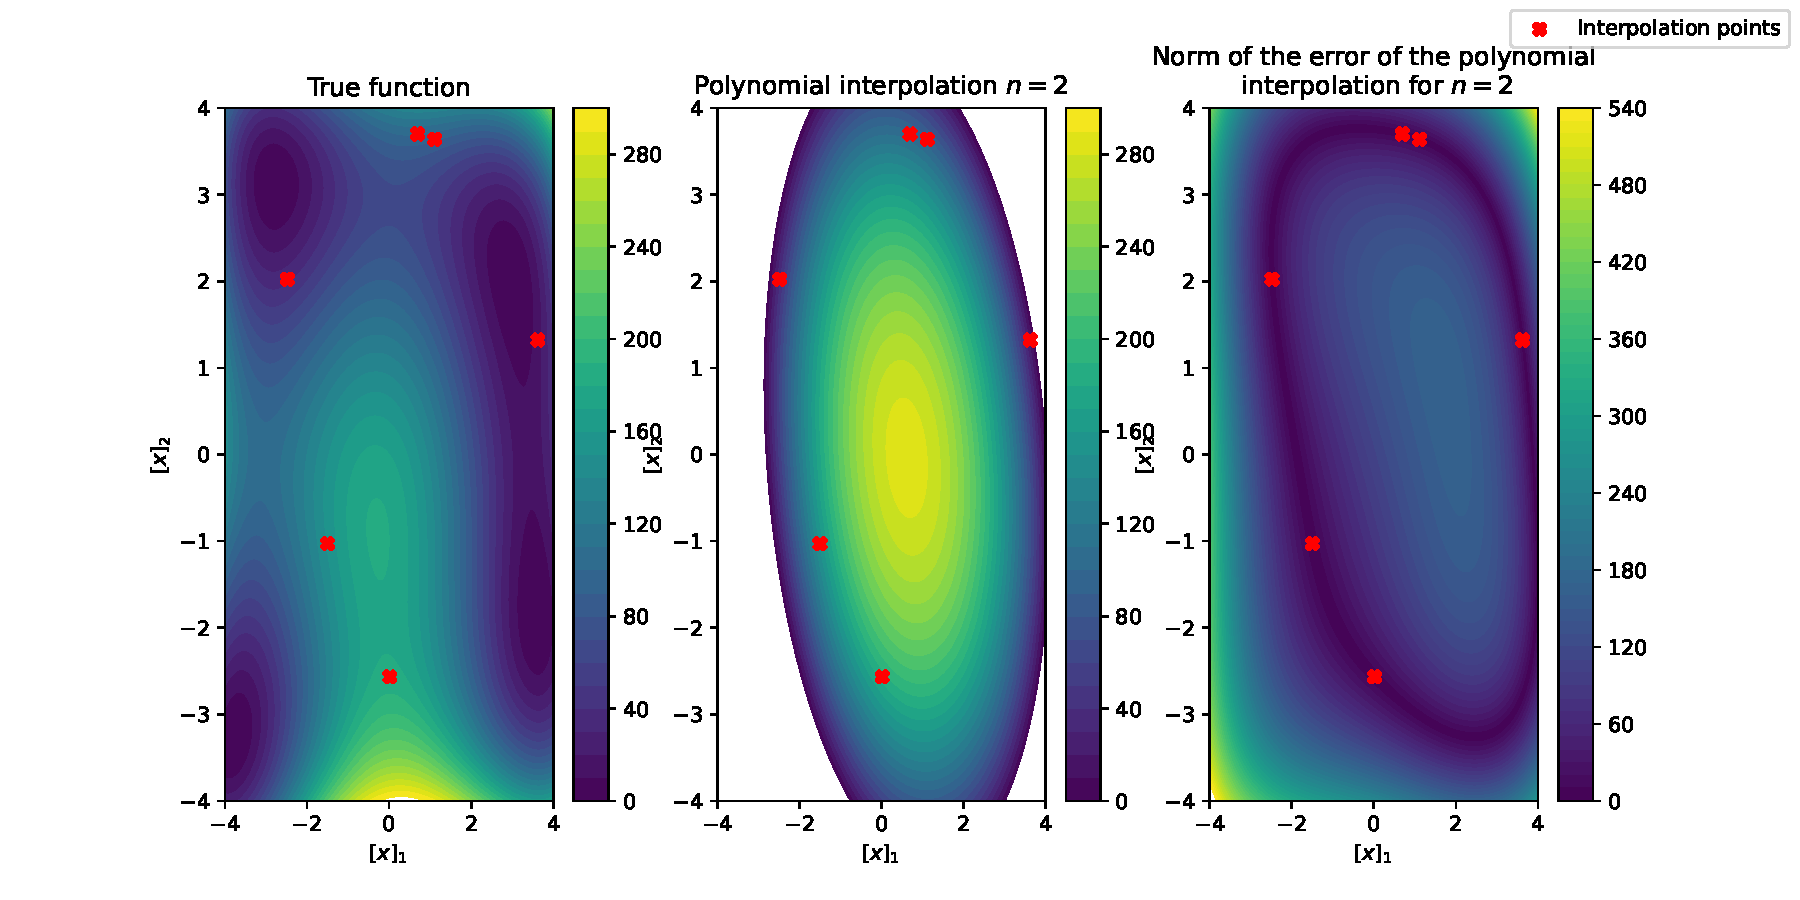
\includegraphics[width=0.7\linewidth]{homework1/polynomial_interpolation_2.pdf}
    \end{figure}
    \begin{figure}[H]
        \centering
        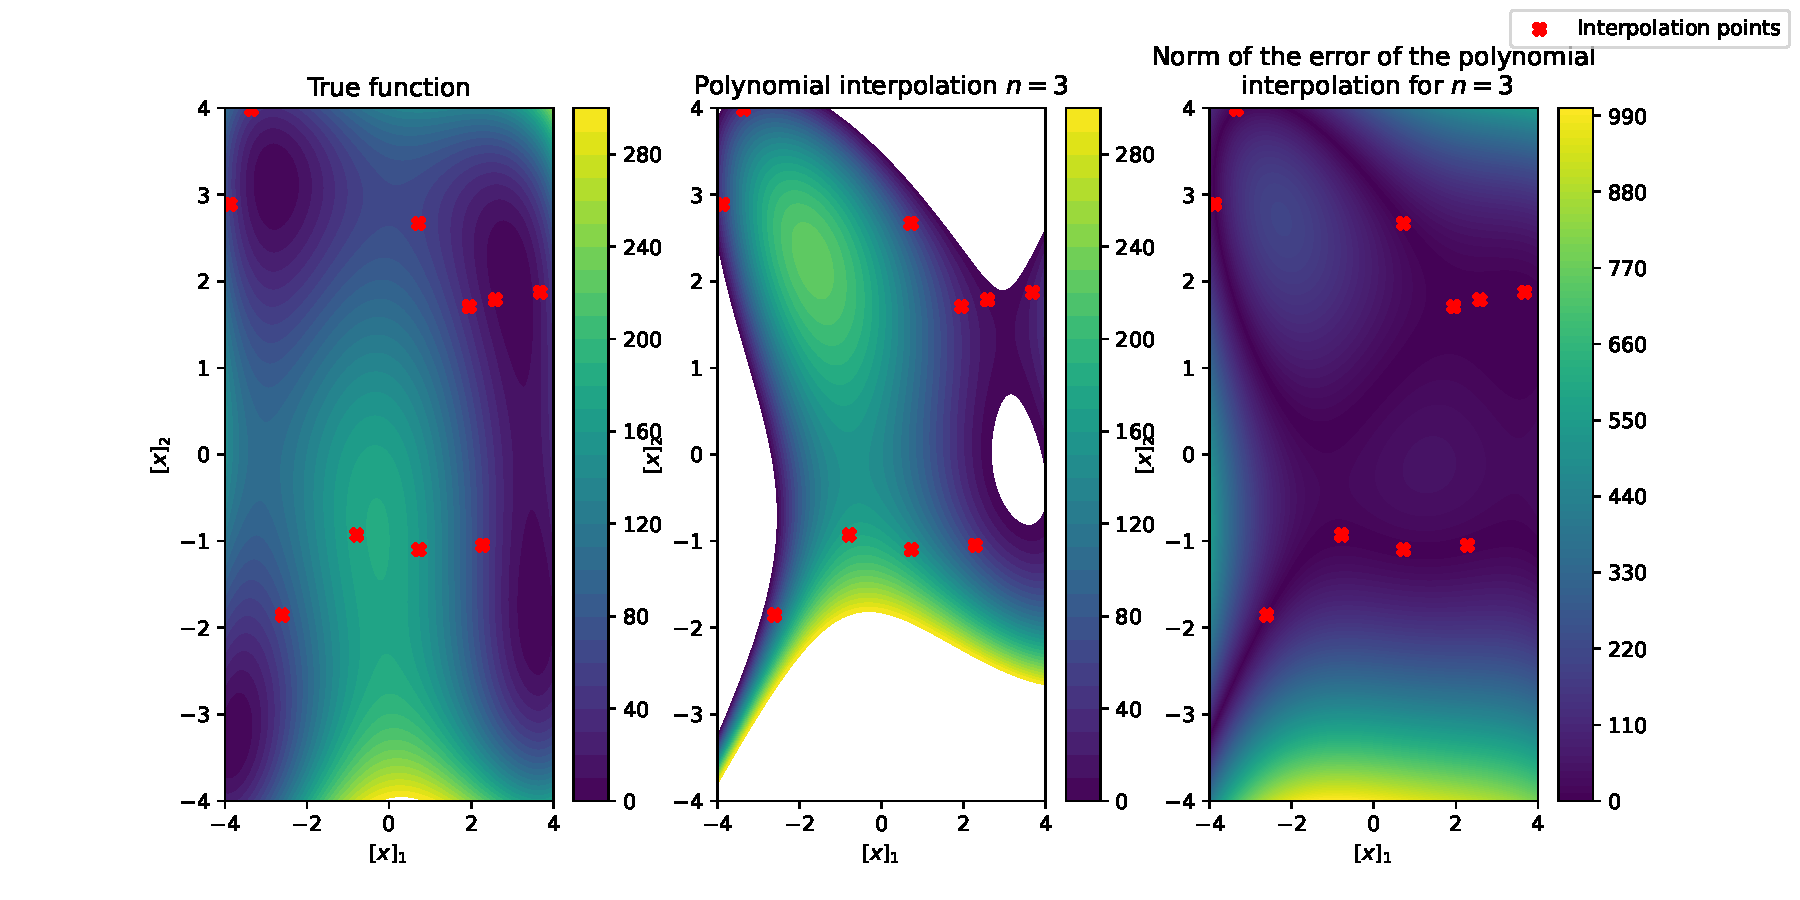
\includegraphics[width=0.7\linewidth]{homework1/polynomial_interpolation_3.pdf}
    \end{figure}
    With low degree interpolation polynomials, the interpolation is quite good around the points of \(\chi\) and the curves connecting them, but can become bad even at small distance from the points in some directions.\\
    With higher degree interpolation polynomials, the interpolation becomes better, until the number of parameters in the system is sufficient to fit exactly the given function \(f\).
    \begin{figure}[H]
        \centering
        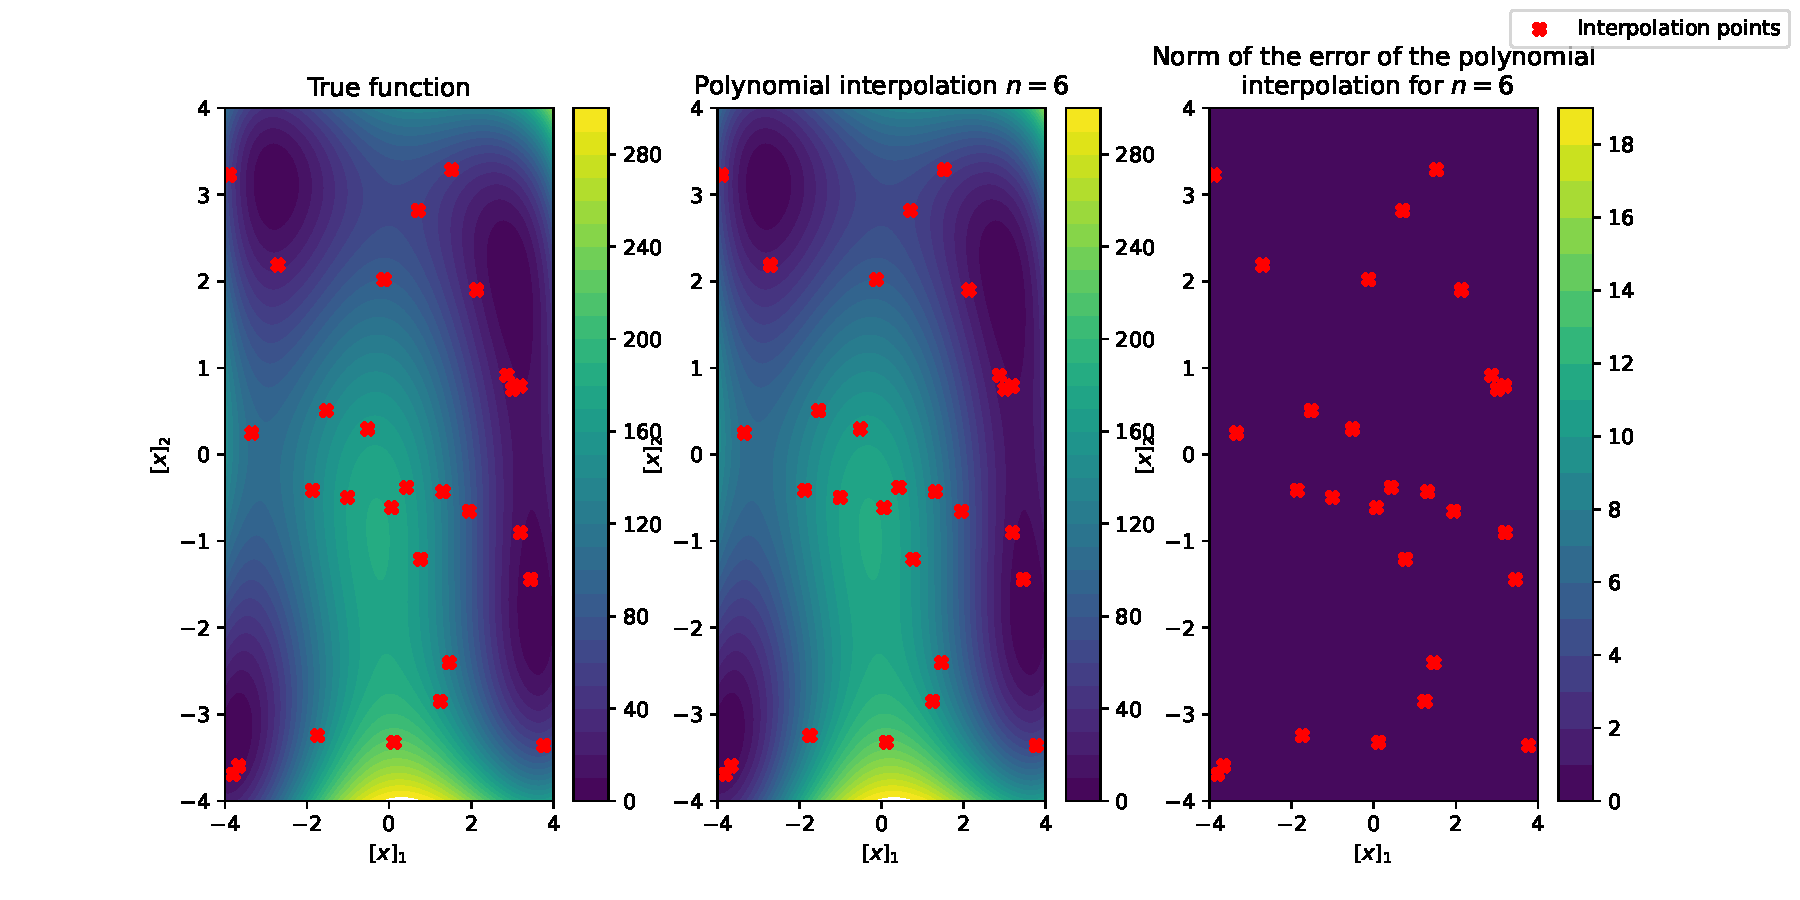
\includegraphics[width=0.7\linewidth]{homework1/polynomial_interpolation_6.pdf}
    \end{figure}
\end{tcolorbox}
\begin{tcolorbox}[breakable,
                  colback=white,
                  colframe=white!75!black,
                  title={Study the effect of scaling (affine transformation with \(A = hI\), \(h > 0\) and \(b = 0\)) on the conditioning of the Vandermonde matrix. More precisely, display on the same graph, for different values of \(n\ge 0\), the condition numbers of \(V_{h\chi_n}\) as a function of \(h\), with a logarithmic y-scale.}
                 ]
    \begin{figure}[H]
        \centering
        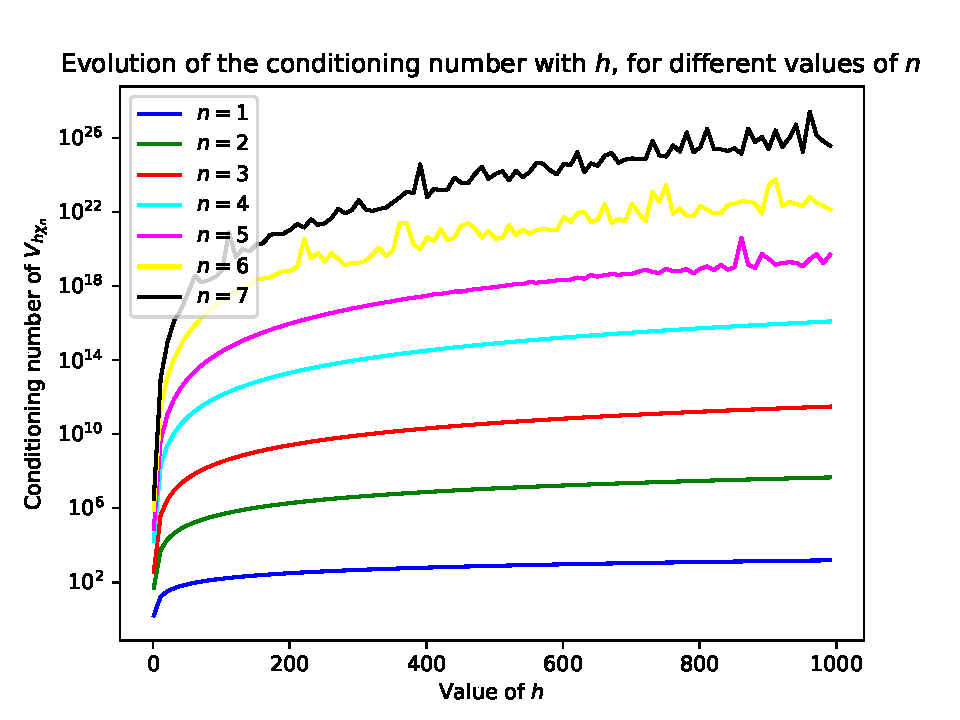
\includegraphics[width=0.7\linewidth]{homework1/scaling.pdf}
    \end{figure}
    The condition number is a measure of the "sensitivity" of the system to a small change in the input, i.e. the set \(\chi\). We can see on the graph hereabove that it becomes very high very fast as the degree of the polynomial is raised\footnote{The oscillations on the upper values are due to roundup errors above \(10^{-16}\).}. For a given value of \(n\) however, it grows fast for small values of \(h\) and then seems to reach a plateau. Considering what it represents, the values reached in this problem are very high and would tend to indicate an ill-posed problem even for relatively small values of \(n\). 
\end{tcolorbox}
\end{document}